\documentclass{article}
\usepackage{graphicx}
\usepackage[fontsize=11pt]{scrextend}
\title{PowerEnjoy Service - Project Plan}
\usepackage{float}

\begin{document}

\subsection{Schedule}
In this chapter we are going to provide the general schedule of principal tasks that we will perform to complete our project. The tasks chosen are essential for completeness of project, that is mean we have not consider the trivial process into a single tasks and the more details will be define during the project.\\
The entire process is fallow the phases of waterfall model, therefore dependencies between core activities are sequential. Moreover, to avoid delay caused by tasks waiting for another to complete, we will anticipate the start of the task as much as possible. \\
For readability, we have split in two part, the first one cover the Feasibility study and RASD and DD, and, due to dependency between activities the second part starting from the end of DD to the end of project.\\ 
The detail duration estimation will be found in the next chapter. 

\begin{figure}[H]
\centering
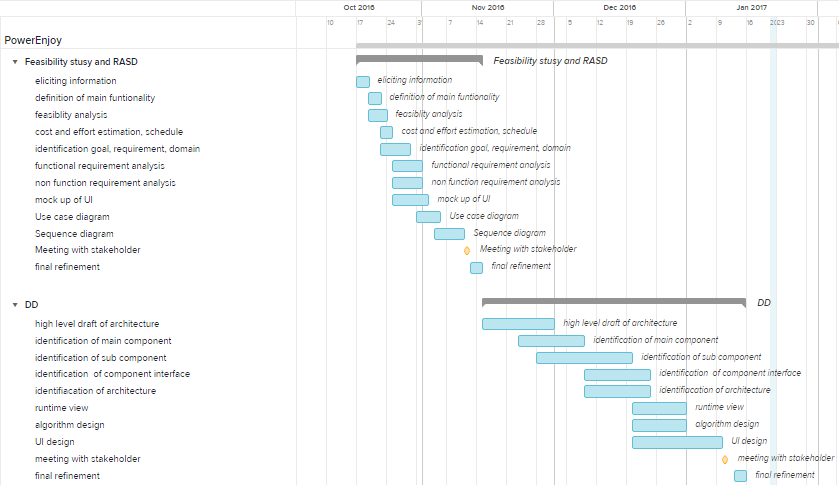
\includegraphics[width=1.2\textwidth]{schedule1.png} 
\end{figure}

\begin{figure}[H]
\centering
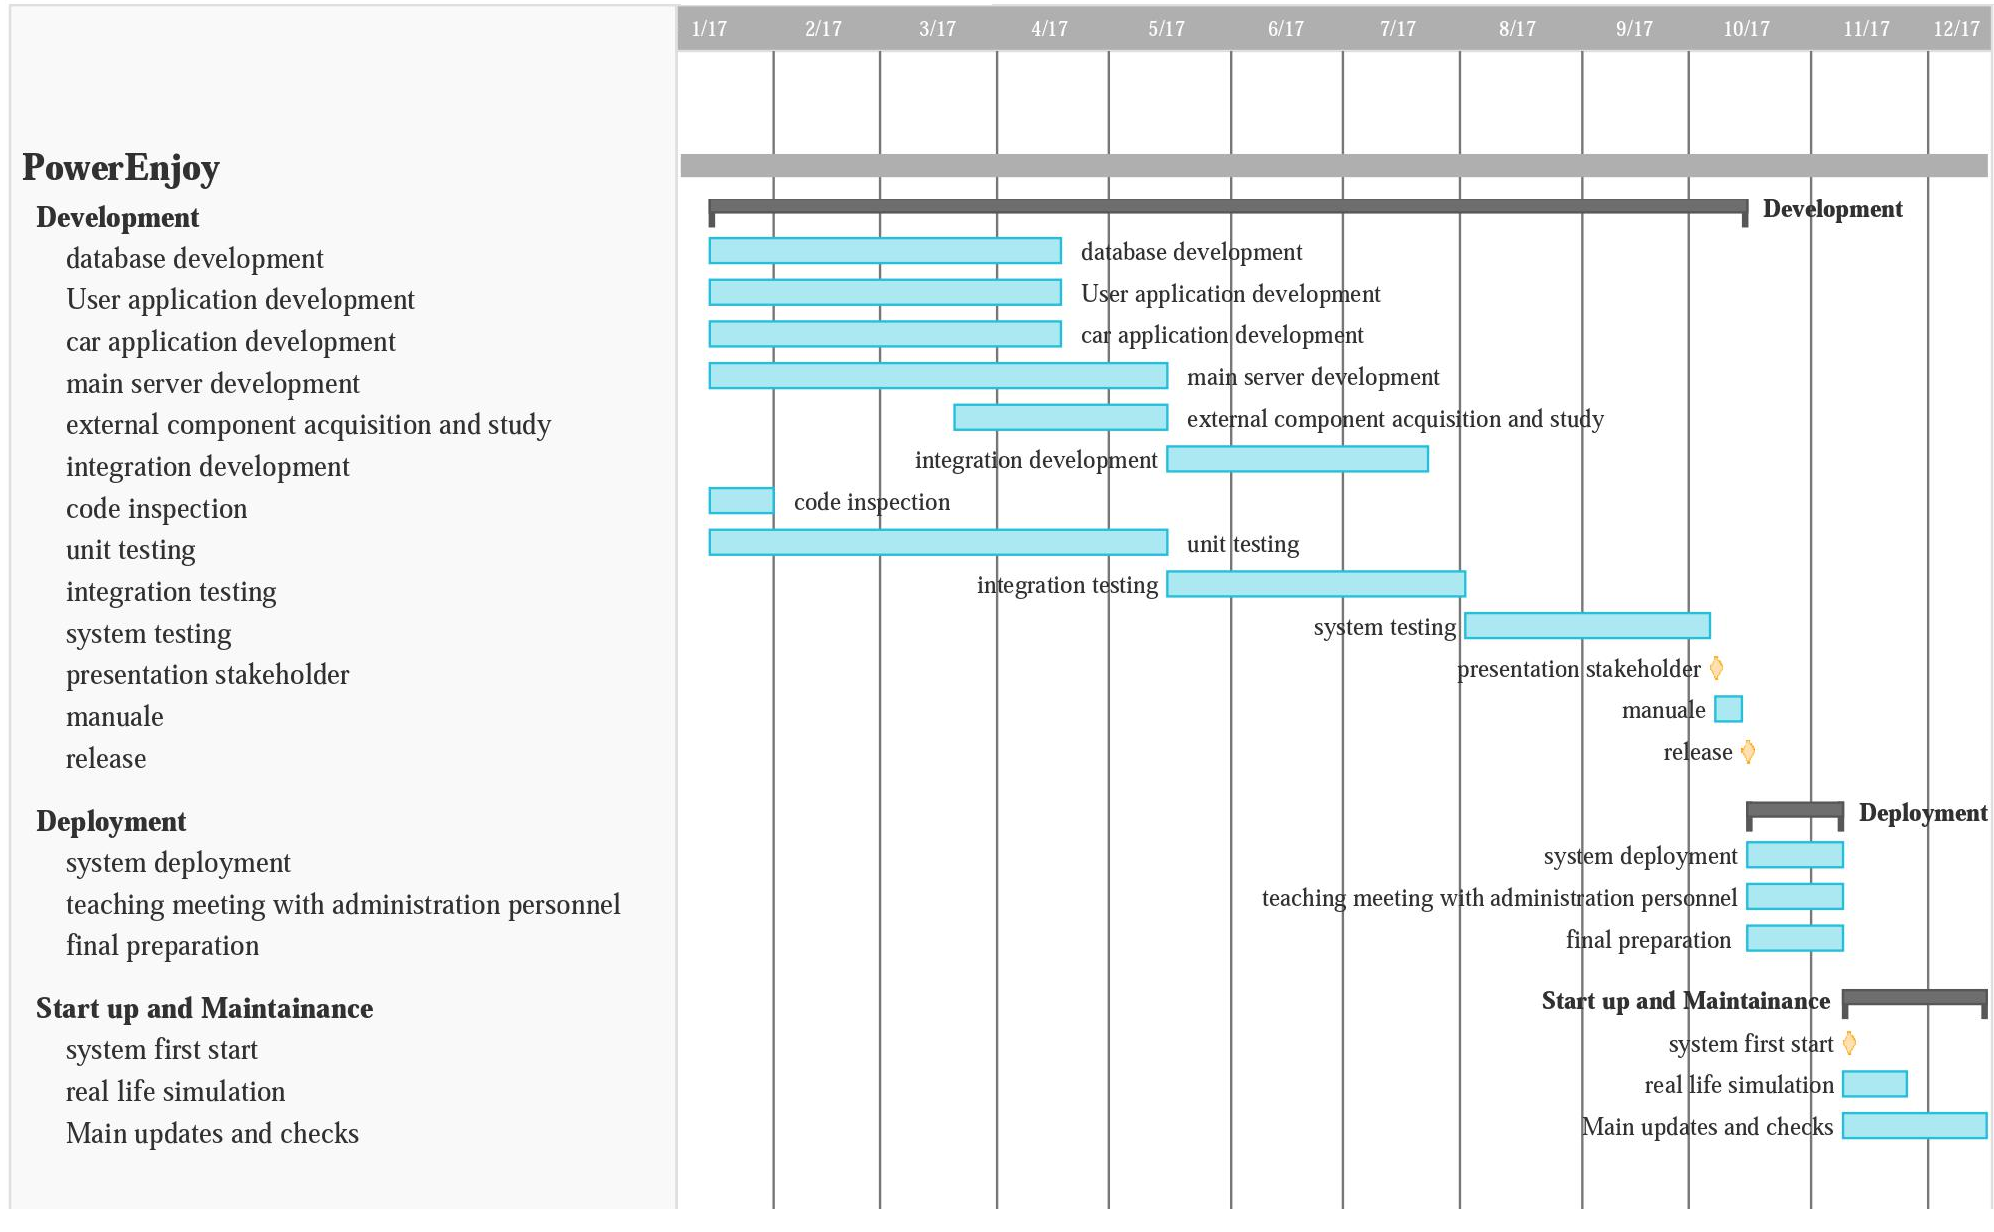
\includegraphics[width=1.2\textwidth]{schedule2.png} 
\end{figure}

\newpage
\subsection{Resource allocation}
In this chapter we going to continue the discourse of how to divided the work between development team. The table below is show the duration and who will be assigned as responsible person of each task.\\ Aforementioned person will organize detail human resource allocation of the a single task assigned, aiming to guarantee the complete within the deadline. So we not to provide the specific staff allocation chart.

\begin{figure}[H]
\centering
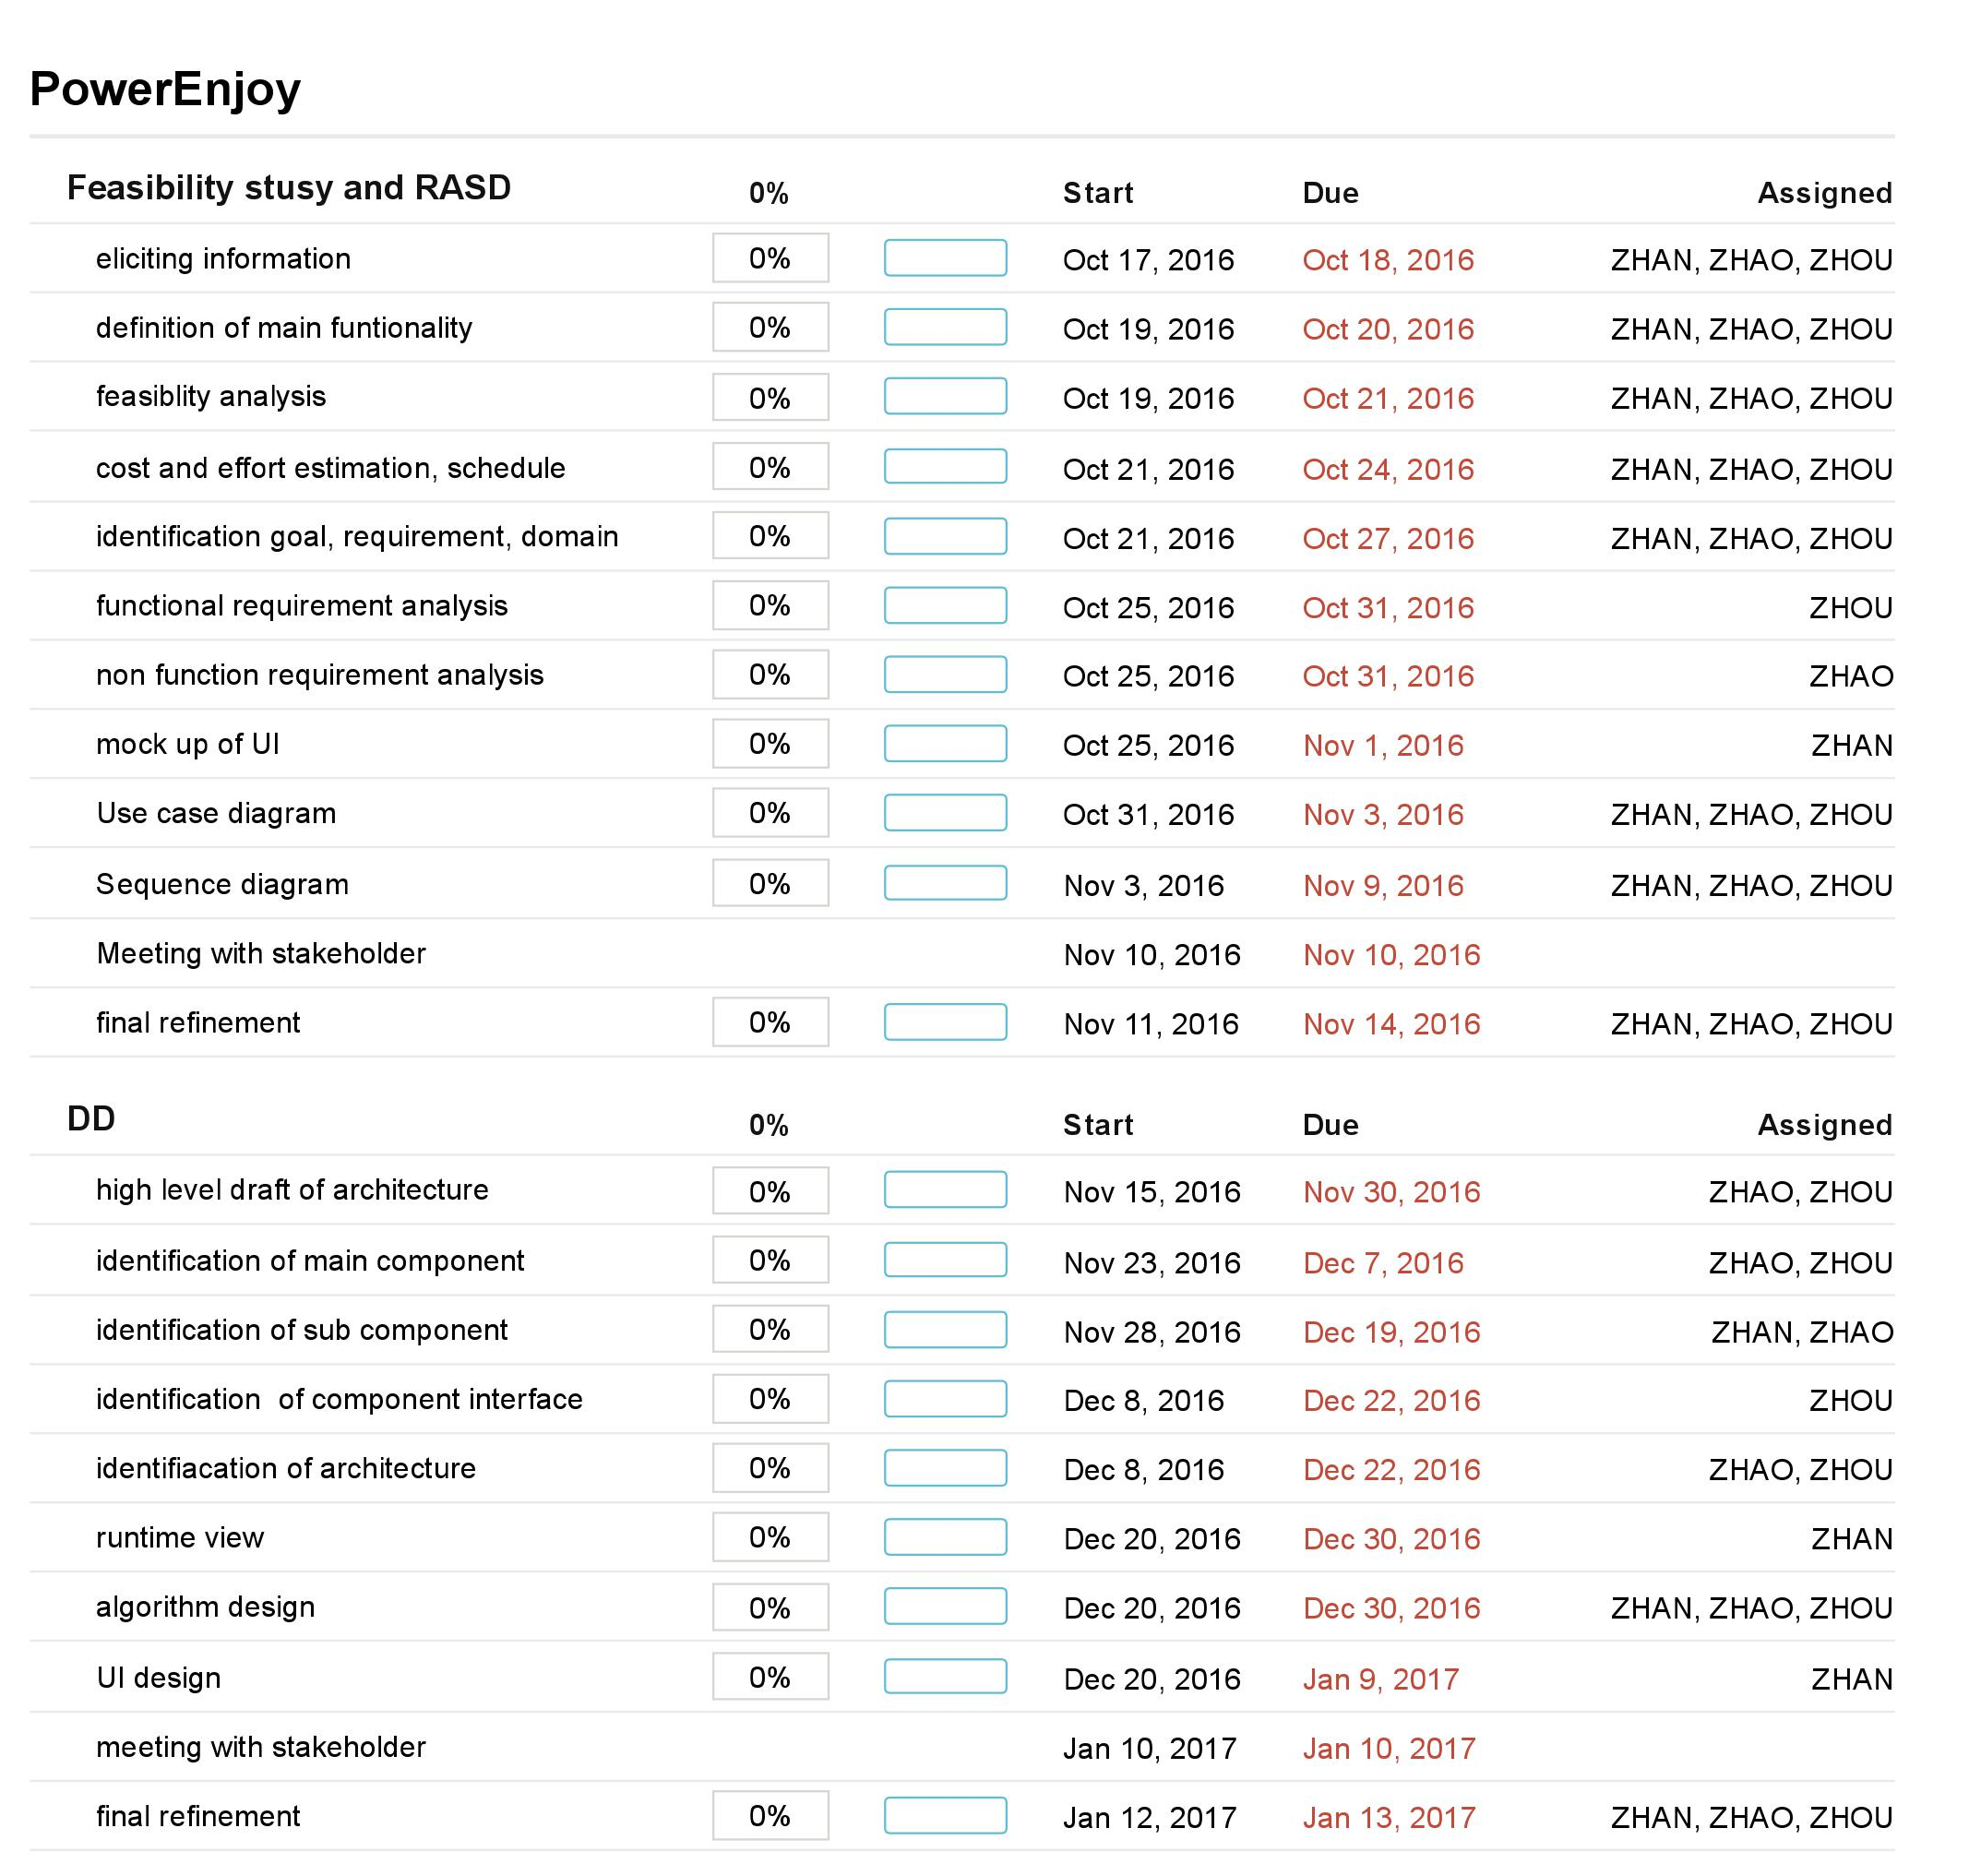
\includegraphics[width=\textwidth]{resource1.png} 
\end{figure}

\newpage
\begin{figure}[H]
\centering
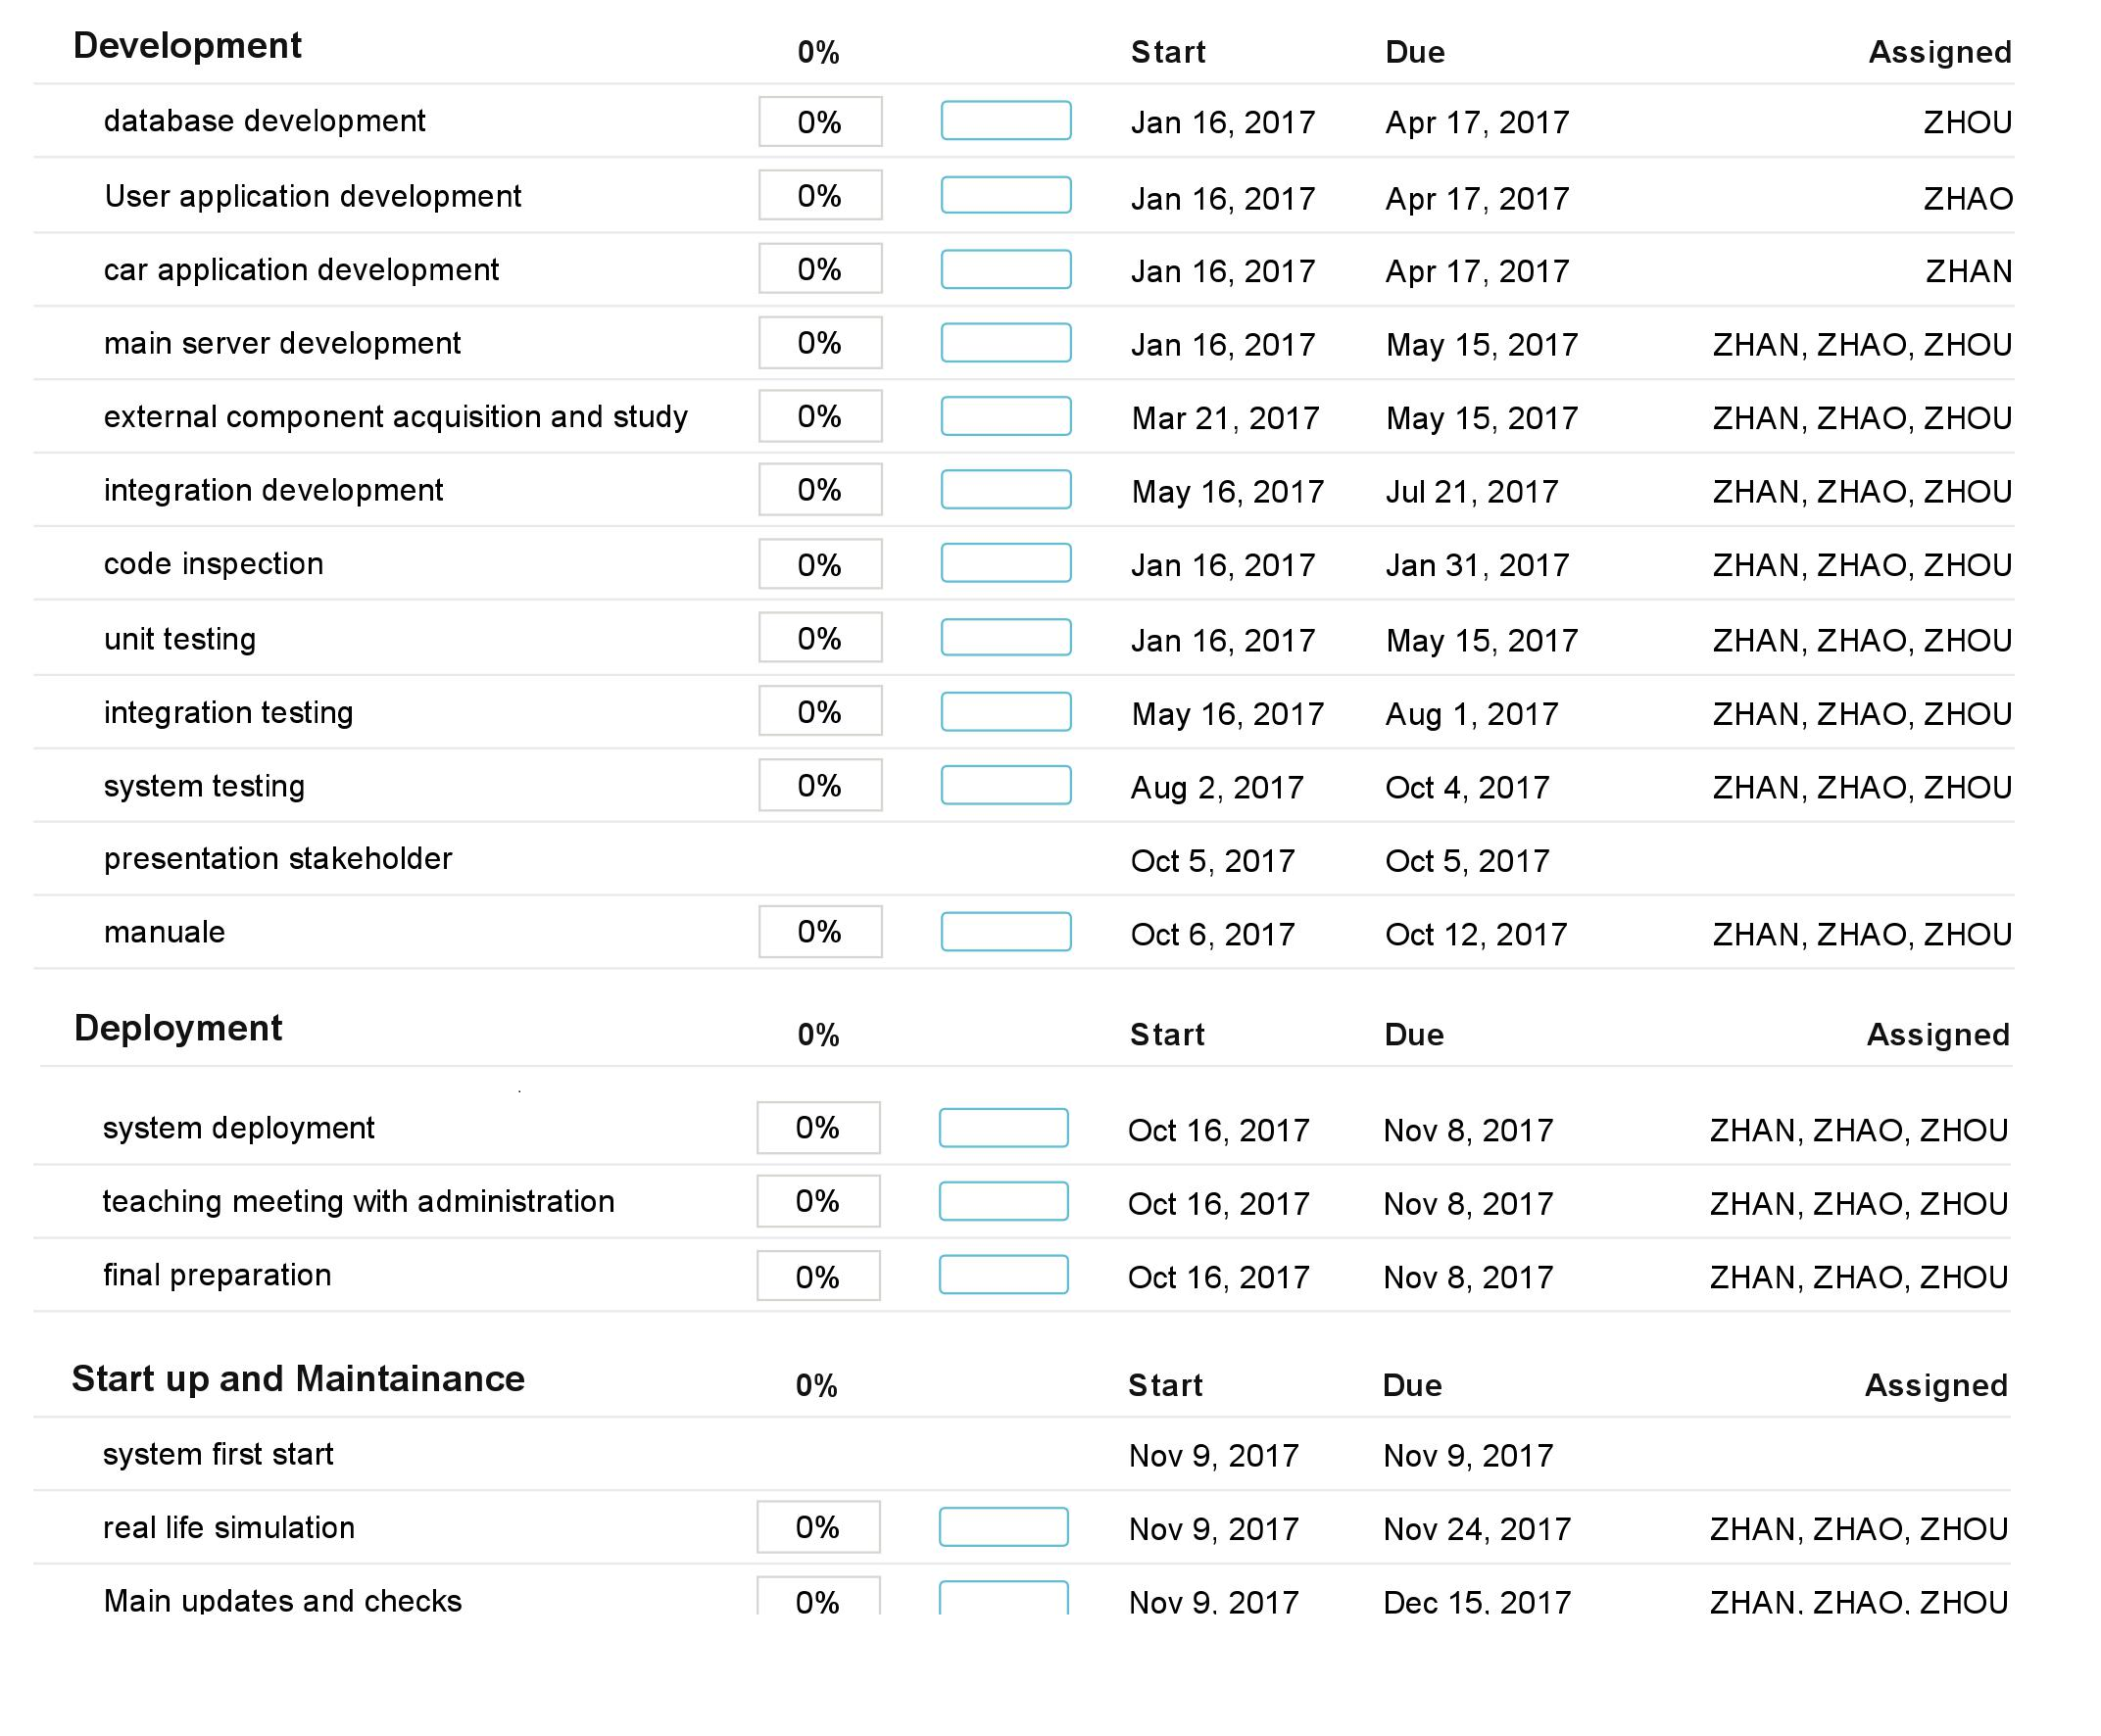
\includegraphics[width=\textwidth]{resource2.png}   
\end{figure}
\end{document}
